\documentclass[aps]{revtex4-2}

\usepackage{graphicx}
\usepackage[dvipsnames]{xcolor}
\usepackage{tikz}
\usetikzlibrary{quantikz}
\usepackage{amsmath, amsthm, amssymb, mathtools}
\usepackage{fancyhdr}
\usepackage{geometry}
\usepackage{bm}
\usepackage{subfig}
\usepackage{multirow}
\usepackage{array}
\usepackage{hyperref}

\newtheorem{theorem}{Theorem}

\pagestyle{plain}




% \fancyheadoffset{-0.001\textwidth}
% \pagestyle{fancy}
\setlength{\textwidth}{7in}
\setlength{\evensidemargin}{-0.2in}
\setlength{\oddsidemargin}{-0.2in}
\setlength{\headheight}{14pt}
%\setlength{\headwidth}{6in}
\setlength{\topmargin}{-0.5in}
\setlength{\textheight}{8.4in}
% \setlength{\baselineskip}{10pt}


\begin{document}
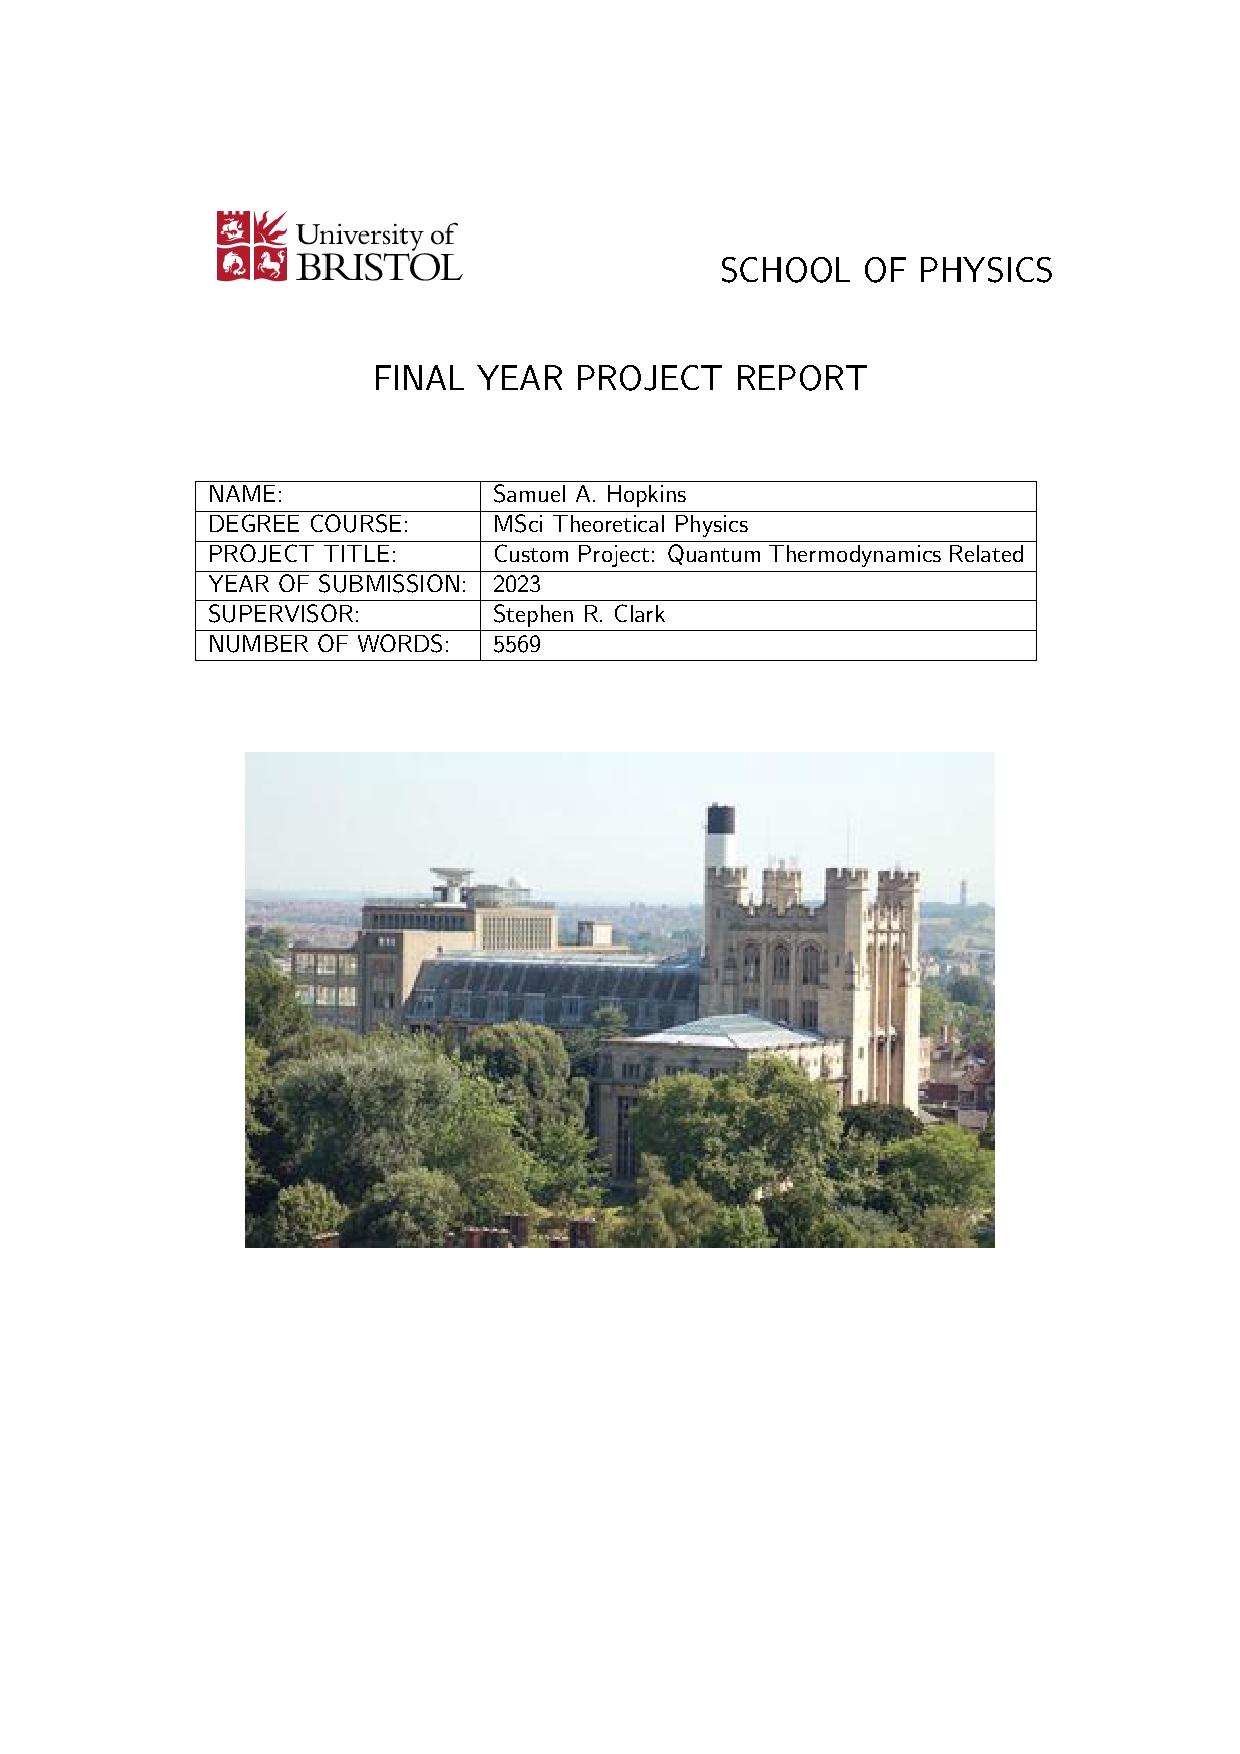
\includegraphics[width = \textwidth]{preface.pdf}
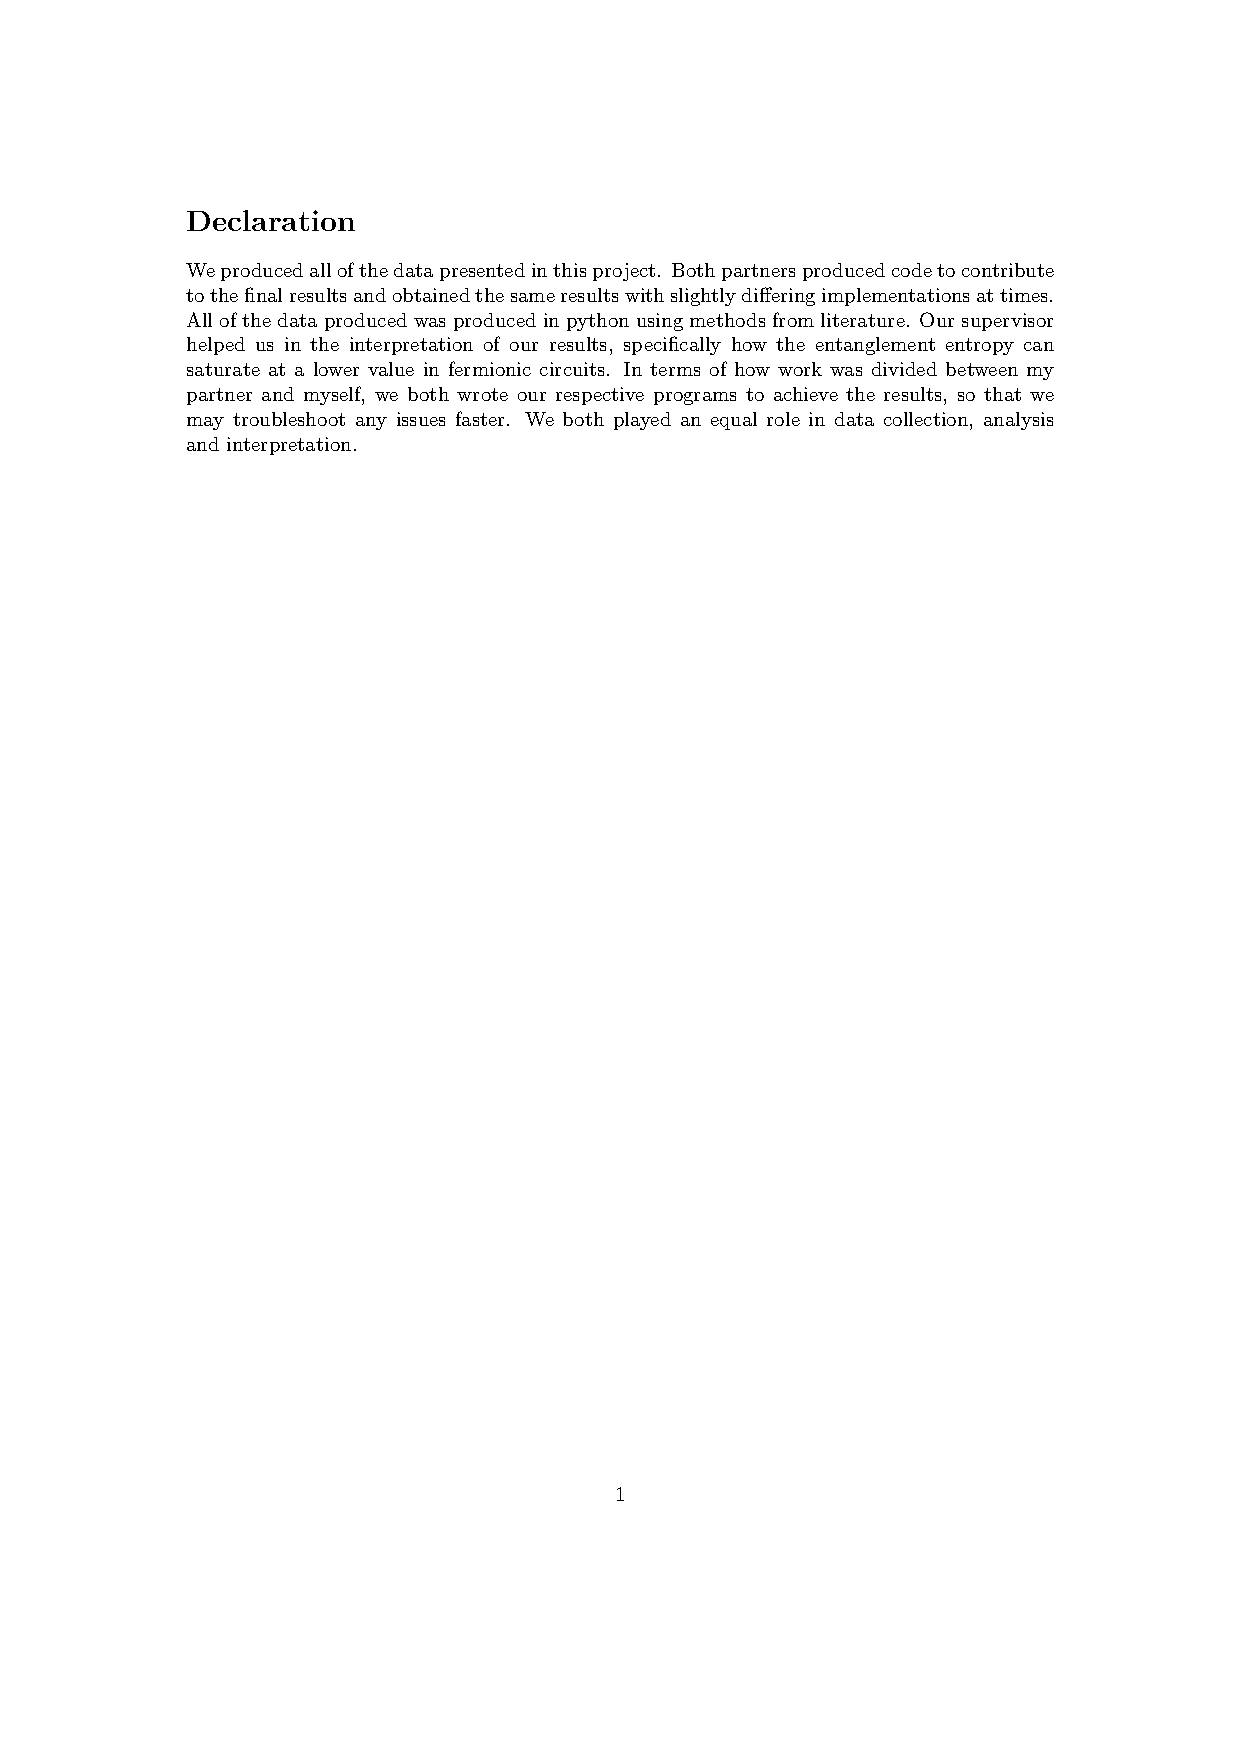
\includegraphics[width = \textwidth]{Report_Latex_template__1_.pdf}
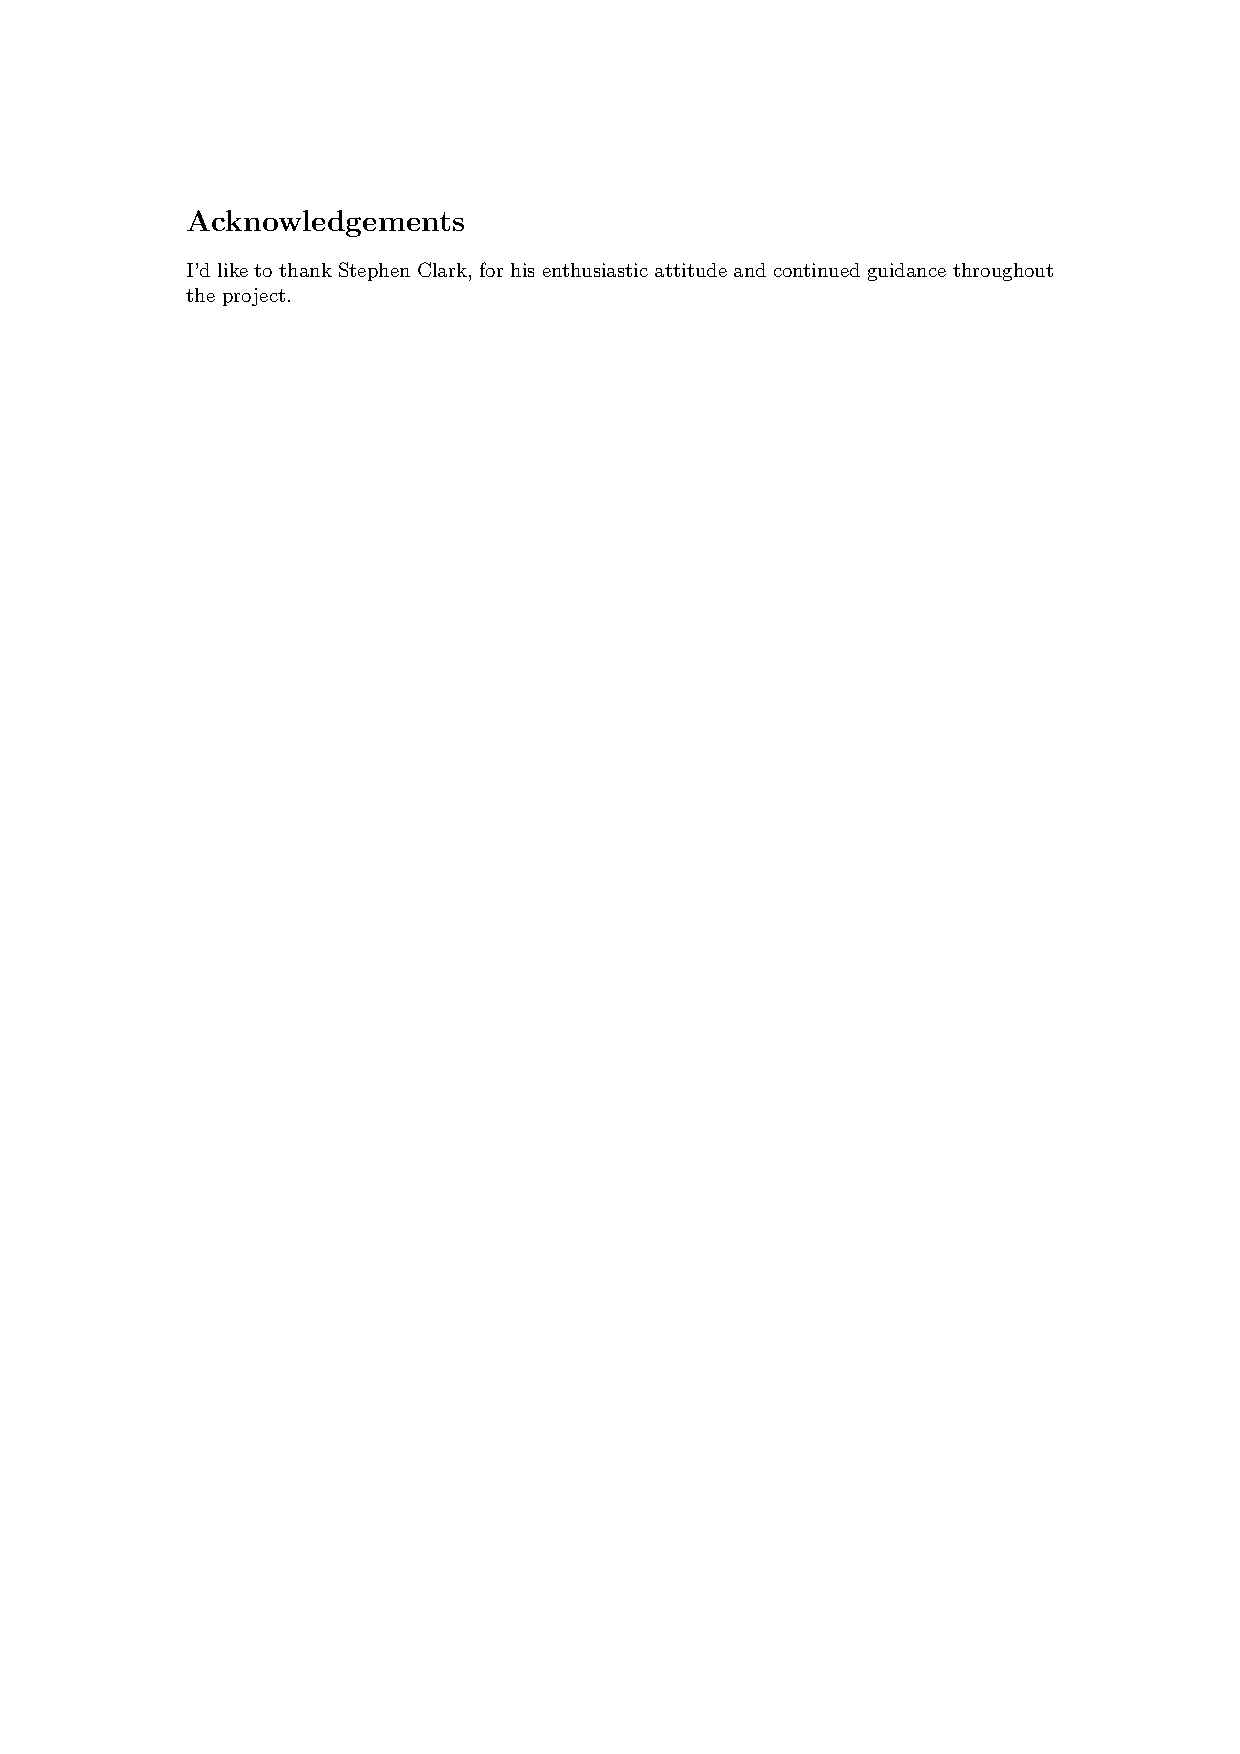
\includegraphics[width = \textwidth]{ackno.pdf}
% 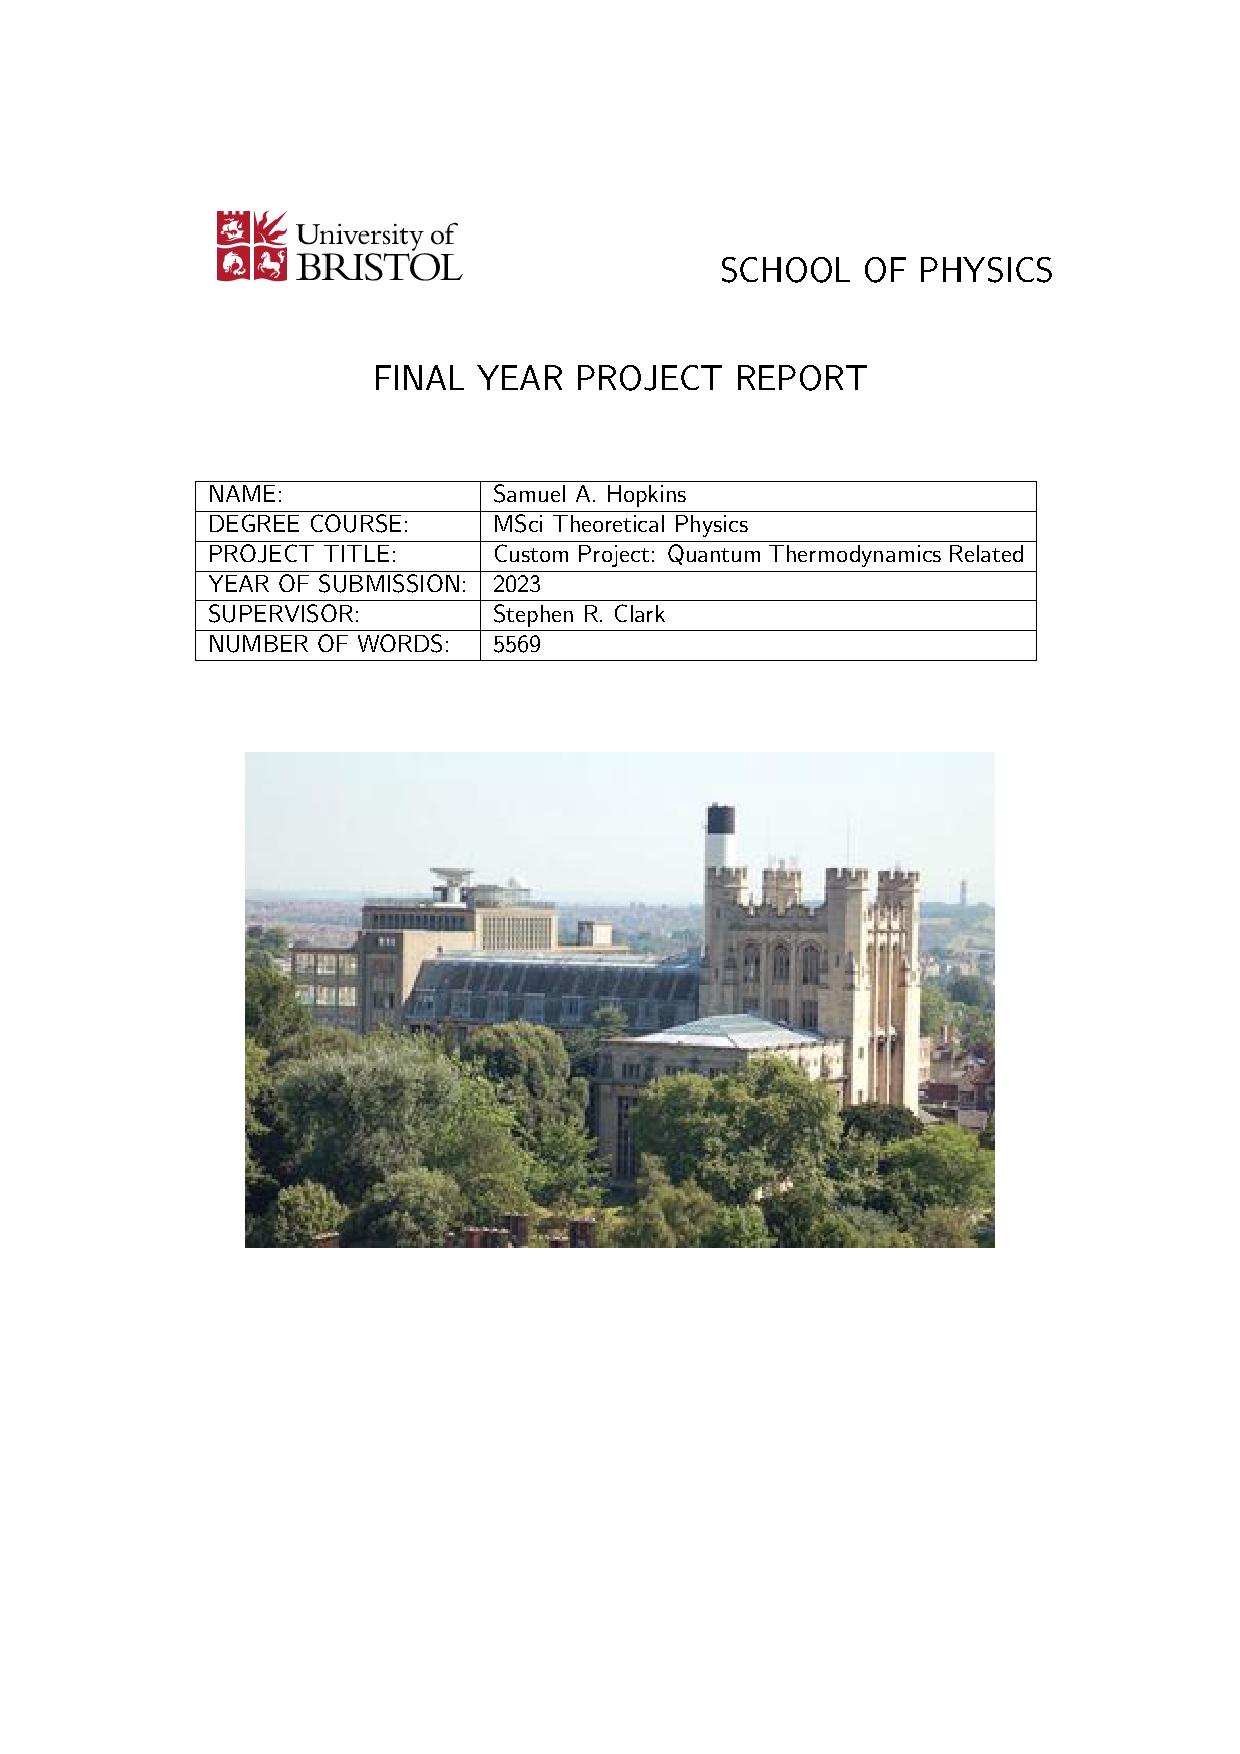
\includepdf[pages=-]{preface.pdf}

\title{Quantum Scrambling}

\author{Samuel A. Hopkins$^{1*}$}
\affiliation{$^1$H. H. Wills Physics Laboratory, University of Bristol, Bristol, BS8 1TL, UK}
\date{\today}
\thanks{Email: cn19407@bristol.ac.uk\\
Supervisor: Stephen R. Clark\\
Word Count: 5569
}
\begin{abstract}
    Using atypical quantum circuit models, specifically super-Clifford and non-interacting fermion circuits, we explore the dynamics of operator space entanglement entropy and the process known as scrambling. In super-Clifford circuits, we reproduce the work from Blake and Linden, and achieve a maximal entanglement entropy using the stabilizer formalism. We find that no local operators can generate non-trivial entanglement dynamics within super-Clifford circuits. By using non-interacting fermion circuits we show that fermionic systems subject to random unitary circuits exhibit weak entangling dynamics in operator space, with it's entanglement entropy saturating at a fraction of the Page value.
\end{abstract}
\maketitle



% \clearpage
% \tableofcontents



%%INTRODUCTION Outline:
% Introduce quantum scrambling - short short description
%where and why is it being studied 
% Explore the limitations
%Collect key results to simulate dynamics
% 
% \section{Report Plan}
%     \subsection{Introduction}
%         \begin{itemize}
%             \color{ForestGreen}
%             \item Introduce quantum scrambling with a short description
%             \item Where and why is this being studied
%             \item What are the uses and conclusions we can draw - state examples 
%             \item What are our aims
%             \item Outline the structure of the report
%         \end{itemize}






%Images
% Random UNitary circuit





\section{Introduction}




\section{Quantum Information and Computation}


\newpage
\section{Qubit Systems}
\subsection{Quantum Bits} % add some detail about physical relevance and distinguishibility.

In the theory of quantum computation, a quantum bit (qubit) is a spin-$\frac{1}{2}$ particle or a two-level system, in which a single bit of information can be encoded. 
Unlike it's classical counterpart, where a bit occupies a binary state of 0 or 1, a qubit exists in a linear superposition of quantum states, expressed as 
$|\psi\rangle = \alpha |0\rangle + \beta |1\rangle$, where $\alpha$ and $\beta$ are complex probability amplitudes.
The states $|0\rangle$ and $|1\rangle$ form an orthonormal basis in the simplest Hilbert space, $\mathbb{C}^2$, and are known as computational basis states. 
To extend this description to a system with 2 or more qubits, the use of the tensor product is required. For example, consider two subsystems
$A$ and $B$, with their respective Hilbert spaces, $\mathcal{H}_{A}$ and $\mathcal{H}_{B}$ such that they each describe a single qubit. 
The total Hilbert space, $\mathcal{H}_{AB}$ for the two-qubit, is constructed from $\mathcal{H}_{A}$ and $\mathcal{H}_{B}$, as
\begin{equation}
    \mathcal{H}_{AB} = \mathcal{H}_{A} \otimes \mathcal{H}_{A}.
\end{equation}
To generalise, the Hilbert space of an $n$ qubit system is written as, 
\begin{equation}
    \mathcal{H} = \mathcal{H}^{\otimes n} \equiv \mathcal{H}_{1} \otimes \mathcal{H}_{2} \otimes \dots \otimes \mathcal{H}_{n}. 
\end{equation}
The many-qubit states that span $\mathcal{H}$ are constructed identically, and are often expressed as a binary strings for a given configuration, 
\begin{equation}\label{nqubit}
    |x_1\rangle \otimes |x_2\rangle \otimes \dots \otimes |x_n\rangle \equiv |x_1 x_2 \dots x_n\rangle.
\end{equation}





\subsection{Quantum Circuits}

The overarching aim of this *report* focuses on how many body systems, e.g an $n$ qubit system, as described above, 
evolves in time. The evolution of a quantum system is described by a unitary transformation, that maps an initial configuration, $|\psi_0\rangle $
to a time-evolved configuration $|\psi\rangle$ as follows, 
\begin{equation}
    |\psi \rangle = U |\psi_0\rangle. 
\end{equation}
Where $U$ is some unitary operator, $UU^{\dagger} = U^{\dagger}U = I$. 
In the context of qubit systems, unitary evolution may be deconstructed into a sequence of linear transformations acting on a finite subregion of the Hilbert space. 
This results in an intuitive description of many-body dynamics, where evolutions are represented as a circuit diagrams, 
with each time step in the unitary evolution corresponding to a quantum logic gate action upon a set of qubits.
This is analogous to classical computation, where circuits are comprised of logic gates acting on bit-strings of information. 
In contrast, quantum logic gates are linear operators that have a distinct matrix representation \footnote{Any linear map between two finite dimensional vector spaces, in this case finite dimensional Hilbert spaces, may be represented as a matrix. }.  

Each quantum logic gate has a specified gate symbol, as can be seen in Fig. \ref{Paulis}, allowing the creation of complicated quantum circuitry that can be directly
mapped to simple matrix manipulations.

\begin{figure}[h]
    \centering
    \begin{subfloat}[pauliX]{
        \centering
        \begin{quantikz}
            &  \gate{X} 
                &  \qw
        \end{quantikz}
    }
    \end{subfloat}
    \hspace{10pt} 
    \begin{subfloat}[pauliY]{
        \centering
        \begin{quantikz}
            & \gate{Y}
                & \qw
        \end{quantikz}
    }
    \end{subfloat}
    \hspace{10pt} 
    \begin{subfloat}[pauliZ]{
        \centering
        \begin{quantikz}
            & \gate{Z}
                & \qw
        \end{quantikz}
    }
    \end{subfloat}
\end{figure}

The gates shown in Fig. \ref{Paulis} are  the Pauli operators, equivalent
to the set of Pauli matrices, $P \equiv \{X, Y, Z\}$ for which $X, Y \text{ and } Z$ are defined in their matrix representation as
\begin{align}
    \label{PauliMatrices}
    X = \begin{bmatrix}
            0 & 1 \\
            1 & 0
        \end{bmatrix},
     &  &
    Y = \begin{bmatrix}
            0  & -i \\
            i & 0
        \end{bmatrix},
     &  &
    Z = \begin{bmatrix}
            1 & 0  \\
            0 & -1
        \end{bmatrix},
\end{align}

These gates are all one-qubit gates, as they only act upon a single qubit.
Together with the Identity operator, $I$, the Pauli matrices form an algebra, such that they 
satisfy the following relations:
\begin{align}
    XY = iZ,  &  & YZ = iX,  &  & ZX = iY,  \\
    YX = -iZ, &  & ZY = -iX, &  & XZ = -iY,
\end{align}
\begin{align}
    X^2 = Y^2 = Z^2 = I.
\end{align}


The set of Pauli matrices and the identity form
the Pauli group, ${\cal P}_n$, defined as the $4^n$ $n$-qubit tensor products of the Pauli matrices (\ref{PauliMatrices}) and the
Identity matrix, $I$, with multiplicative factors, $\pm 1$ and $\pm i$ to ensure a legitimate group is formed under multiplication.
For clarity, consider the Pauli group on 1-qubit, ${\cal P}_1$:
\begin{equation}
    {\cal P}_1 \equiv \{ \pm I, \pm iI, \pm X, \pm iX \pm Y, \pm iY, \pm Z, \pm iZ\}.
\end{equation}



From this, another group of interest can be defined, namely the Clifford group, ${\cal C}_n$, defined as a
subset of unitary operators that normalise the Pauli group *INSERT CLIFFORD GROUP DEFINITION*.
Notable elements of this group are the Hadamard, Controlled-Not and Phase operators.

The Hadamard operator, $H$ maps computational basis states to a superposition of computational basis states, written explicitly 
in it's action as, 
\begin{align*}
    H|0\rangle = \frac{|0\rangle + |1\rangle}{\sqrt{2}}, && H|1\rangle = \frac{|0\rangle - |1\rangle}{\sqrt{2}},
\end{align*}
or in matrix form, 
\begin{equation}
    H = \frac{1}{\sqrt{2}} \begin{bmatrix}
        1 & 1\\
        1 & -1
    \end{bmatrix}.
\end{equation}

Controlled-NOT, $CNOT_{AB}$, is a controlled two-qubit gate. The first qubit, $A$ acts as a `control' for an operation to be 
performed on the target qubit, $B$. It's matrix representation is, 
\begin{align*}
    CNOT_{12} = \begin{bmatrix}
        1 & 0 & 0 & 0 \\
        0 & 1 & 0 & 0 \\
        0 & 0 & 0 & 1 \\
        0 & 0 & 1 & 0
        \end{bmatrix}
\end{align*}

The Phase operator, denoted $R$ is defined as,
\begin{align*}
    R =
    \begin{bmatrix}
        1 & 0                  \\
        0 & e^{i\frac{\pi}{2}}
    \end{bmatrix}.
\end{align*}

\subsection{Entanglement in Qubit Systems}

The CNOT operator is often used to an generate entangled state. One such state is the maximally entangled 2-qubit state,
called a Bell state, $|{\bm\Phi}^{+}\rangle_ = (|00\rangle + |11\rangle)/\sqrt{2}$. This is prepared
from a $|00\rangle$ state, by applying a Hadamard to the first qubit, and subsequently a Controlled-Not gate:
\begin{itemize}
    \item[I.] $H \otimes I |00\rangle = \left (\frac{|0\rangle + |1\rangle }{\sqrt{2}}\right )|0\rangle$ 
    \item[II.]  $CNOT \left (\frac{|0\rangle + |1\rangle }{\sqrt{2}}\right )|0\rangle = \frac{|00\rangle + |11\rangle}{\sqrt{2}}$
\end{itemize}
% \begin{align}
%     H \otimes I |00\rangle = \left (\frac{|0\rangle + |1\rangle }{\sqrt{2}}\right )|0\rangle \\
%     CNOT \left (\frac{|0\rangle + |1\rangle }{\sqrt{2}}\right )|0\rangle = \frac{|00\rangle + |11\rangle}{\sqrt{2}}
% \end{align}
The corresponding circuit representation of this preparation is given in Fig. \ref{Bellstate}.

\begin{figure}
    \centering
    \begin{quantikz}
        \lstick{$\ket{0}$} & \gate{H} & \ctrl{1} & \qw\rstick[wires=2]{$\ket{\Phi^+}$} \\
        \lstick{$\ket{0}$}& \qw & \targ{} & \qw
    \end{quantikz}
    \caption{Preparation of a Bell state from $\ket{0}$ using a Hadamard and CNOT.}
    \label{Bellstate}
\end{figure}
The output Bell state, cannot be written in product form. That is, the state cannot be written as,
\begin{align*}
    |{\bm\Phi}^+\rangle = & \left[ \alpha_0 |0\rangle + \beta_0|1\rangle\right] \otimes \left[\alpha_1 |0\rangle + \beta_1|1\rangle\right] \\
    =                     & \alpha_0\beta_0 |00\rangle + \alpha_0\beta_1|01\rangle + \alpha_1\beta_0|10\rangle + \alpha_1\beta_1|11\rangle
\end{align*}
since the $\alpha_0$ or $\beta_1$ must be zero in order to ensure the $|01\rangle$, $|10\rangle$ vanish.
However, this would make the coefficients of the $|00\rangle$
or $|11\rangle$ terms zero, breaking the equality. Thus, $|{\bm\Phi}^+\rangle$ cannot be written in
product form and is said to be entangled. This defines a general condition for a arbitrary state to be entangled 
\cite{nielsen_chuang_2010}.


% To give an example, consider the preparation of a GHZ state, $\frac{|000\rangle + |111\rangle}{\sqrt{2}}$ 
% from an initial all-zero state, $|000\rangle$. This transformation may be written as, 
% \begin{align*}
%    |\psi_{GHZ}\rangle = U |000\rangle,\\
%    |\psi_{GHZ}\rangle = (CNOT_{13})(CNOT_{12})(H\otimes I \otimes I)|000\rangle. 
% \end{align*}
% Where $I$ is the identity operator. As a circuit diagram, the transformation takes the following form: 
%    \begin{center}
%     \begin{quantikz}
%         \lstick{$\ket{0}$} & \gate{H} & \ctrl{1} & \ctrl{2} & \qw\rstick[wires=3]{$\ket{\psi_{GHZ}}$} \\
%         \lstick{$\ket{0}$}& \qw & \targ{} & \qw & \qw\\
%         \lstick{$\ket{0}$}& \qw & \qw & \targ{} & \qw
%     \end{quantikz}
%     % \caption{Preparation of a Bell state from $\ket{0}$ using a Hadamard and CNOT.}
% \end{center}

%%%%%%%%%%%%%%%






%can perform operations on qubits in a similar fashion to logical operations on bits, since maps are linear we can express them as matrices. introduce some operators. 
%then explain how we may form a quantum circuit from these. 
%then explain how we encode information



\section{Fermionic Systems}


%Indistinguishibility. 

The familiar qubit system may be mapped onto a system of identical particles (fermions), such that the 
overall many body state describing the system, is invariant under particle exchange. This is 
performed via a Jordan-Wigner transformation, which maps any local spin-model to a local fermionic model \cite{10.1093/acprof:oso/9780199573127.001.0001}.
To gain an understanding of how this can be carried out and why it is relevant, it will be useful to introduce the core concepts and language from \textit{Second Quantization}.
\subsubsection{Second Quantization and Indistinguishable Particles}
The wave function for a system of $N$ identical particles is $\psi(x_1, x_2, \dots x_N)$, where a particle is specified by it's position vector, $\vec{x}$. For bosonic systems, the wavefunction is symmetric under particle exhchange, while fermionic systems present anti-symmetric wavefunctions under particle exchange called Slater determinants. 

The construction of the $n$ particle state via the extension of the single particle wavefunction, as described in (\refeq{nqubit}), 
leads to a redundancy in it's description of a many-body state and an unnecessarily large Hilbert space.
A more efficient appraoch to describing many-body states is found in the formalism of second quantisation. Instead of describing states with Slater determinants, a \textit{Fock state} presents an elegant and convinient basis in which to work in. The Fock state of a many-body system is represented in an occupancy number basis, written as $|n_1, n_2, \dots, n_L\rangle$, where $n_i$ is the occupation number of a given local fermionic mode (LFM). For systems of bosonic particles,  the occupancy can take any real non-negative integer. For systems of many fermionic particles, the occupancy number is either $0$ or $1$ with no two fermions ever occupying the same mode.

To preserve the symmetric properties of Fock states, second quantization introduces fermionic creation and annihilation operators. The creation operator, $a^{\dagger}_{i}$ creates a particle at site $i$ if unoccupied, and the annihilation operator, $a_i$, removes a particle at site $i$ if occupied. More formally, it's action on a Fock state may be written as, 
\begin{align}
    a_j^{\dagger} |n_0, \dots, n_j, \dots, n_{m-1}\rangle = {(-1)}^{\sum^{j-1}_{s=0}n_s} (1-n_j) |n_0, \dots, n_j - 1, \dots, n_{m-1}\rangle, \\
    a_j |n_0, \dots, n_j, \dots, n_{m-1}\rangle = {(-1)}^{\sum^{j-1}_{s=0}n_s} n_j |n_0, \dots, n_j - 1, \dots, n_{m-1}\rangle.
\end{align}
With the fermionic creation and annihilation operators obeying crucial anti-commutation relations:
\begin{align}
    \{a_j, a_k\} \equiv \{a_j^{\dagger}, a_k^{\dagger}\} = 0, && \{a_j, a_k^{\dagger}\} = \delta_{jk}I.
\end{align}

Using these operators, an arbitrary Fock state, $|\psi_{F}\rangle$ of $L$ modes, may be prepared from a set of creation operators acting on the vacuum, $|\Omega\rangle = |0, 0 \dots, 0\rangle$, 
\begin{equation}
    |\psi_{f}\rangle = (a_{1}^{\dagger})^{n_1} (a_{2}^{\dagger})^{n_2} \dots (a_{L}^{\dagger})^{n_{L}}|{\Omega}\rangle.
\end{equation}

\subsubsection{Jordan-Wigner Transformation}

Using the fermionic operators, the Jordan-Wigner transformation may be defined, which maps a system of $N$ spin-$\frac{1}{2}$ particles onto a system of $N$ `spinless' fermions by defining the fermionic operators in terms of the Pauli spin operators \cite{landahl2023logical}, 
\begin{align}
    a^{\dagger}_i = \left(\prod^{i-1}_{k = 1} Z_k\right) \sigma^{-}_{i}, &&
    a_i = \left(\prod^{i-1}_{k = 1} Z_k\right) \sigma^{+}_{i}.
\end{align}
Where $\sigma^{\pm}_{j} = (X_j \pm i Y_j)/2$.
Such a mapping allows the Hilbert space of $N$ qubits to be identified with the Hilbert space of $N$ local fermionic modes (LFM's). However this transformation is non-local, with fermionic operators having support over the almost the entire Hilbert space of $N$ qubits \cite{ Ba_uls_2007}. 


As an alternative description, the \textit{Majorana operators} may be defined as 
$c_{2k} = a_k + a_k^{\dagger}$ and $c_{2k+1} = i(a_k^{\dagger} - a_{k})$ for $k =  1, \dots, N$ such that they satisfy $\{c_j, c_k\} = 2\delta_{jk}$. This description splits each LFM in two, increasing the number of modes to $2N$. 





\section{Scrambling Dynamics}
\subsection{Random Unitary Circuits}
To study the generic quantum many-body systems, random unitary circuits provide a minimally structured model that can emulate the required dynamics of generic or `chaotic' unitary evolutions.\cite{https://doi.org/10.48550/arxiv.2210.10129}.
In the study of operator hydrodynamics The set-up is a chain of $L$ spins, labelled as $q = 0, 1, \dots, L-1$ each with their respective local dimension $h$ and is subject to a random unitary circuit $\mathcal{U}$. The total circuit is constructed per timestep, by acting with a layer of 2-qubit unitaries on evenly-bonded spins, followed by a layer of unitaries applied to odd-bonded spins. More formally, each timestep in the circuit corresponds to an action by $U = U_{\text{even}} U_{\text{odd}}$, where $U_{\text{even}}$ is given by the tensor product of individual 2-qubit unitaries $U_{q, q+1}$ applied to all evenly bonded sites, $q, q+1$ for $q$ even,  and $U_{\text{odd}}$ is given by the tensor product of individual 2-qubit unitaries $U_{q, q+1}$ applied to all odd bonded sites, $q, q+1$ for $q$ odd. Each 2-qubit unitary acts on nearest neighbour spins, and is drawn from the uniform (Haar) probability distribution on the unitary group $U(4)$ or from a specific subgroup \cite{hunterjones2018operator}.
For our purposes, we require a simpler model. For a system of $L$ qubits, each time step corresponds to a randomly drawn unitary acting on a randomly drawn qubit, $q_i$ and it's nearest neighbour, $q_{i+1}$.

% such as the Clifford group, $\mathcal{C} \equiv \{H, CNOT, R\}$.

To extract solvable dynamics and utilise well-estabilished measures, information about the state of the system is encoded as strings of operators. A convinient basis to work with in qubit systems is found in the set of Pauli matrices.
For example, a system with $L = 5$ spins could be represented by the operator string $\mathcal{O} = I \otimes I \otimes P_i \otimes I \otimes I$, where $P_i$ is an arbitrary Pauli matrix. An operator of this form is a \textit{local} operator, as it only acts non-trivially on a single site. 
For a system subject to generic unitary evolution , we expect that information encoded by an initially simple product operator to spread over the large number of degrees of freedom becoming highly complicated sum of global operators, such that they have support over the entire system. This process is known as Quantum Scrambling, and can be regarded as the combined notion of \textit{Operator Spreading} and a growth in \textit{Operator complexity}. 

\subsection{Operator Spreading} 
To give a picture of operator spreading, this section will primarily focus on the evolution of Pauli strings. Starting from some initially local product operator, such as 
$\mathcal{O} = \mathbb{1} \otimes\dots \otimes \mathbb{1} \otimes \sigma_{x} \otimes \mathbb{1} \otimes \dots \otimes \mathbb{1}$. This system will evolve via $|\psi (t)\rangle = U |\psi_0\rangle$ and the operator string will evolve via the Heisenberg evolution of operators, 
\begin{equation}\label{heisenberg_evolution}
    \mathcal{O}(t) = U(t) \mathcal{O} U^{\dagger}(t).
\end{equation}
 Following this evolution, the local operator with minimal support, $O_j$ has evolved to $O_j(t)$ with support over a
large region of sites \cite{Khemani_2018}. Operators that grow in this way, will spread ballistically \cite{Roberts_2015, Lieb:1972wy, Schuster_2022} and are often
characterised by the out-of-time ordered correlator (OTOC) \cite{Xu2022} and the square-commutator\cite{Blake_2018}. This also gives an
intuitive picture of operator spreading, with the squared commutator defined as 
\begin{equation}
  C(t) = \langle [O(t), V_i][O(t), V_i]^{\dagger}\rangle
\end{equation}
where $V_i$ is a static local operator at site $i$ \cite{https://doi.org/10.48550/arxiv.1804.08655}. Then at $t=0$, $O(t)$
acts on a single site or a finite region of sites, such that it commutes with the static operator, $V_i$ and $C(t) = 0$.
Once the operator spreads, and becomes more non-local, the commutator increases as it's support overlaps with $V_i$.


\subsection{Operator Complexity and Entanglement Entropy}
A key component in quantum supremacy lies in a quantum algorithm's ability to utilise the abudant \textit{entanglement} within a system. In simple bipartite systems, where $\mathcal{H}_{AB} = \mathcal{H}_{A}\otimes \mathcal{H}_{B}$, the state of this system, $|\Psi_{AB}\rangle \in \mathcal{H}_{AB}$ is 
said to be entangled if and only if the state cannot be written in product form, $|\Psi_{AB}\rangle =  |\Psi_{A}\rangle \otimes |\Psi_{B}\rangle$, where $|\Psi_{A}\rangle$ and $|\Psi_{B}\rangle$ are the two vectors corresponding to the Hilbert spaces of each subsystem. If the state $|\Psi_{AB}\rangle$ is not entangled, then it is a product state and is said to be separable \cite{Horodecki_2009}.
 

\subsubsection{Entanglement In Qubit Systems}
Qubit systems provide the simplest decription of entangled states in bipartite systems. For a system of two qubits, there exist 4 specific maximally entangled configurations, called Bell states: 

\begin{align}\label{bellpair}
    |\Phi^{+}\rangle = \frac{|00\rangle + |11\rangle }{\sqrt{2}}, && |\Phi^{-}\rangle = \frac{|00\rangle - |11\rangle }{\sqrt{2}},
    \\
    |\Psi^{+}\rangle = \frac{|01\rangle + |10\rangle }{\sqrt{2}}, && |\Psi^{-}\rangle = \frac{|01\rangle - |10\rangle }{\sqrt{2}}.
\end{align}
We can verify that the state, $|\Phi^{+}\rangle $ is an entangled state by writing, 
\begin{align}\label{entangle}
    |{\Phi}^+\rangle &=  \left[ \alpha_0 |0\rangle + \beta_0|1\rangle\right] \otimes \left[\alpha_1 |0\rangle + \beta_1|1\rangle\right], \\
    &=                      \alpha_0\beta_0 |00\rangle + \alpha_0\beta_1|01\rangle + \alpha_1\beta_0|10\rangle + \alpha_1\beta_1|11\rangle.
\end{align}
We require that the $\alpha_0$ or $\beta_1$ terms must be zero in order to ensure the $|01\rangle$, $|10\rangle$ vanish. However, this would make the coefficients of the $|00\rangle$ or $|11\rangle$ terms zero, breaking the equality. Thus, $|{\bm\Phi}^+\rangle$ cannot be written in product form and is said to be entangled.

\subsubsection{Entanglement In Fermionic Systems}

For a system of indistinguishable particles, each with only one spin degree of freedom (effectively spinless), entanglement can emerge as states analgous to a Bell state (\refeq{bellpair}). Considering a system of 2 modes, occupied by a single indistinguishable particle, a fermion. The state of this system can be expressed as, 
\begin{equation}
    |\psi_{f}\rangle = \frac{|0_{A}\rangle |{1_{B}}\rangle + |1_{A}\rangle |0_{B}\rangle}{\sqrt{2}}.
\end{equation}
Where $A, B$ `label' the two respective modes, and are included to express the state of this system intuitively.
One can easily verify that this state is entangled, as outlined in (\refeq{entangle}), as it cannot be expressed in product form.  However, this definition of entanglement is of little use when working with larger multi-fermion systems. We require entanglement measures to make qualitative statements on the complexity of operators and the systems they represent \cite{Eckert_2002}.

\subsubsection{Entanglement Measures}

For many-body systems, the definition of entanglement cannot be directly used to detect entanglement between states. Instead, entanglement measures provide a useful tool for detecting and analysing entanglement dynamics. In the case of distinguishable particles, one such entanglement measure is the \textit{Schmidt Rank}, derived from the \textit{Schmidt Decomposition}. The Schmidt decomposition states for any state vector, $|\Psi\rangle \in \mathcal{H}$ where $\mathcal{H} = \mathcal{H}_{A} \otimes \mathcal{H}_{B}$, there exists an orthonormal basis $\{|a_i\rangle \otimes |b_j\rangle\}$ such that,
\begin{equation}\label{Schmidt}
    |\Psi\rangle = \sum_{i = 1}^{d_A} \sum_{j = 1}^{d_B} D_{ij} |a_i\rangle \otimes |b_j\rangle.
\end{equation}
Where $d_A$ and $d_B$ are the dimensions of the respective subsystems, $A$ and $B$. The matrix $D$ is a matrix of coefficients with the rank being the Schmidt rank. If the Schmidt rank is of rank one, then the state $|\Psi\rangle$ is a product state \cite{Horodecki_2009}. 

In systems of indistinguishable particles, a similar measure exists in the form of the \textit{Slater Rank criterion}. The Slater Decomposition states that for a system of two fermions, in a $N$-dimensional  space specified by the state vector,
\begin{equation}\label{Slater}
    |\Psi\rangle = \sum_{i, j = 1}^N \omega_{ij} a^{\dagger}_{i}a^{\dagger}_j|\Omega\rangle.
\end{equation}
There exists a unitary transformation, $U$ that block diagonalises the coefficient matrix $\omega$. More explicitly,
\begin{align*}
    \omega' = U\omega U^{T} = \text{diag}[Z_0, Z_1, \dots, Z_r], && Z_i = 
    \begin{bmatrix}
        0 & z_i \\
        -z_i & 0
    \end{bmatrix}.
\end{align*}
Where $z_i >0$ $ \forall i \in 1, \dots, r$ and $Z_0$ is an all-zero matrix of size $(N \times 2r) \times (N - 2r)$. The Slater rank is then the number of non-vanishing block matrices \cite{Schliemann_2001}.

Entanglement measures such as the Schmidt and Slater rank, provide useful criterion for entanglement amongst state vectors. However, our aim is to analyse operator complexity signified by the entanglement in operator space. Thus, entanglement measures such as (\refeq{Schmidt}) and (\refeq{Schmidt}), do not provide the adequate tools to analyse the dynamics operator complexity in exactly solvable models. Instead we utilise an entropy entanglement measure, known as the Von Neumann entropy. For a quantum system described by the density matrix, $\rho$, the the Von Neumann entropy, $S$, is defined in general as, 
\begin{equation}
    S = -\text{Tr}(\rho \ln \rho).
\end{equation}
To determine the entanglement entropy, a bipartition is introduced into the system, so that the entanglement entropy describes to which degree the two subsystems that have been partition are entangled. The entanglement entropy is then, 
\begin{equation}\label{entrop}
    S_A = -\text{Tr}(\rho_A \ln \rho_A) = -\text{Tr}(\rho_B \ln \rho_B).
\end{equation}
Where $\rho_A$ , $\rho_B$ describe the subsystems, $A, B$ \cite{PhysRevA.51.2738}.





% This measure provides a nice introduction to how entanglement measures are constructed in bipartite systems, but are not fit for the purposes of this project. A full description can be found in Appendix (X). 
% For bipartite systems of distinguishable particles, the Schmidt rank, derived from the Schmidt decomposition provides a method in determining whether a many-body state is entangled. 











% \begin{figure}
    \centering
    % \begin{quantikz}[transparent]
    %     \lstick{$q_0$}& \gate[2]{U_{01}} & \qw & \qw & \qw \\
    %     \lstick{$q_1$}& & \gate[2]{U_{12}} & \qw & \qw \\
    %     \lstick{$q_2$}& \gate[2]{U_{23}} &&& \qw\\
    %     \lstick{$q_3$}& \qw &&& \qw
    % \end{quantikz}
    \begin{tikzpicture}
        
    \end{tikzpicture}

    \caption{Preparation of a Bell state from $\ket{0}$ using a Hadamard and CNOT.}
    \label{randomunitarycircuit}
\end{figure}
% Quantum scrambling is the process in which local information encoded by a simple product operator is rapidly spread over a large number of degrees of freedom 

% The information becomes highly non-local and the initial simple product operator becomes a complicated sum of product operators. 


\section{Simulating a Quantum Circuit}


%Computational complexity

The size of quantum systems presents computational challenges due to the exponential size of the Hilbert space. A system of $L$ particles 
would have a $2^L$ dimensional Hilbert space. Simulating a quantum circuit of this size, requires the construction of this exponentially large 
Hilbert space, and since quantum dynamics typically utilize the full $2^L$ dimensional space, a classical computer can typically only simulate 
$L = 10-20$ particles in a given system. Thus, circuits that emulate quantum dynamics and can be simulated efficiently on a classical computer, provide
immensely useful tools in the study of quantum systems. In one dimensional systems, there are three known classically simulable or exactly solvable models; 
Clifford circuits \cite{knillGottesman}; matchgates \cite{Jozsa2008} or non-interacting fermion circuits\cite{Terhal2001}; and dual-unitary circuits \cite{Suzuki_2022}. We pin our focus on the first two, Clifford circuits and non-interacting or free fermion circuits.

\subsection{Clifford Circuits}

The main aim of a classically simulable circuit, is to reduce the total size of the system. Clifford circuits achieve this feat by 
abandoning the state-level description in favour of the operators that \textit{stabilize} them. More explicitly, for an arbitrary quantum 
state vector, $|\psi\rangle$, this state is \textit{stabilized} by an operator $S$ if $|\psi\rangle$ is an eigenvector of $S$ with eigenvalue 1: $S |\psi\rangle = |\psi\rangle$ \cite{stabilizercodes}.
Where $S$ is an $L$ qubit string of tensored Pauli operators. To simulate the time evolution of this system, only the Heisenberg evolution of stabilizers, $U(t)SU(t)^{T} \to S(t) $ needs to be simulated which can be achieved in polynomial time if $U(t)$ consists solely of gates from the Clifford group. This comes as a result of the structure of the Clifford group, as any product Pauli operator under conjugation by a Clifford unitary will always be mapped to another product of Pauli operators, by definition.
%Clifford map pauli prods to pauli prods

To implement this numerically, a $(L \times 2L)$ check matrix or stabilizer tableau is created, to encode the stabilizers and their dynamics. The stabilizer tableau, $\mathcal{M}$ is constructed for $L$ stabilizers, which act stabilize a state vector for $L$ qubits, ordered as $q_1, \dots, q_i, \dots, q_L$. The $ith$ row is constructed as follows: if the stabilizer $S_i$ acts with the identity on the $j$th qubit, it's value in the stabilizer tableau is 0. If $S_i$ acts with $\sigma_{x}$, on the $j$th qubit, the $[i,j]$ value in $\mathcal{M}$ is 1, if $S_i$ acts with $\sigma_{y}$, on the $j$th qubit, the $[i,j]$ and $[i, j+L]$ values in $\mathcal{M}$ are 1. If $S_i$ acts with $\sigma_{z}$, on the $j$th qubit, the $[i,j+L]$ value in $\mathcal{M}$ is 1. As an example, consider the Pauli string $ \mathbb{1} \otimes \sigma_{y} \otimes \sigma_{x} \otimes \sigma_{z}$, which will be encoded in a stabilizer tableau as, 
\begin{align*}
     \mathbb{1} \otimes \sigma_{y} \otimes \sigma_{x} \otimes \sigma_{z} \to [0 1 1 0| 0 1 0 1].
\end{align*}  
While Clifford circuits offer no constraint on the amount of entanglement within a system at a state-level description, we cannot expect the same for an operator-level description.  
Since gates from the Clifford group only map products of Pauli operators to products of Pauli operators, we can expect no operator complexity and hence no entanglement in operator space within Clifford circuits.

\subsection{Blake and Linden's Construction}

Blake and Linden \cite{Blake2020} introduce a family of circuits that recover operator complexity on the space spanned by Pauli operators.
They present a gate-set of 'super-Clifford operators' that generate a near-maximal amount of operator entanglement
within the Pauli operator space, called super-Clifford circuits, when under time-evolution. These super-Clifford operators
remain classically simulable, via an extension of stabilisers to operator space, called 'super-stabilisers'.
Super-Clifford operators 'act' on Pauli operators, via conjugation in the Heisenberg picture.
The first super-Clifford operator in the gate set is denoted as ${\bf Z.H}$, which is identified with a on Pauli operators
conjugation by a Phase gate, $T$:
\begin{align}\label{phasegate}
  T^{\dagger} X T = \frac{X - Y}{\sqrt{2}}, &  & T^{\dagger} Y T = \frac{X + Y}{\sqrt{2}}.
\end{align}
Following this, the operators, $X$ and $Y$ can be changed to a state-like representation, with
$X$ denoted as $[{\mathbf 0}\rangle$ and $Y$ denoted as $[{\mathbf 1}\rangle$. Then the action of $\bf Z.H$
can be written as,
\begin{align}
  {\bf Z.H}[{\bf 0}\rangle = \frac{[{\bf 0}\rangle - [{\bf 1}\rangle}{\sqrt{2}}, \\
  {\bf Z.H}[{\bf 1}\rangle = \frac{[{\bf 0}\rangle + [{\bf 1}\rangle}{\sqrt{2}}.
\end{align}
The second gate in the set of super-Clifford operators, is the {\bf SWAP} gate,
\begin{equation}
  \text{\bf SWAP} [{\bf 01}\rangle = [{\bf 10}\rangle,
\end{equation}
formed from the regular 2-qubit SWAP gate, that swaps two nearest neighbour qubits. It conjugates
Pauli operators in the following way
\begin{equation}
  \text{SWAP}^{\dagger} X_1Y_2 \text{SWAP} = Y_1X_2.
\end{equation}
The third gate, denoted $\bf C3$, acts as a combination of controlled-$\text{\bf Y}$ super-operators,
\begin{align}
  {\bf C3} [{\bf 000}\rangle=  {\bf CY}_{12}{\bf CY}_{13} [{\bf000}\rangle = [{\bf 000}\rangle, \\
  {\bf C3} [{\bf 100}\rangle=  {\bf CY}_{12}{\bf CY}_{13} [{\bf100}\rangle = -[{\bf 111}\rangle.
\end{align}
These three super-operators form the gate set $\{ {\bf SWAP}, {\bf Z.H}, {\bf C3}\}$, which generates entanglement
through unitary evolution in operator space, as this gate set maps Pauli strings to a linear superposition of Pauli strings.
Despite the fact a simple string of Pauli operators can evolve into a sum of potentially exponential operator strings,
the dynamics can be computed classically by extending the formalism of stabilizer states to operator space. 

To calculate the entanglement entropy from the stabilizer tableau, a submatrix, $\mathcal{M}_A$ must be formed by keeping the first $2p$ rows in $\mathcal{M}$, where $p$ is the number of qubits in $\mathcal{M}_A$. The entanglement entropy is then given as, 
\begin{equation}
    S_A = I_A - p.
\end{equation}
Where $I_A$ is the rank of the submatrix $\mathcal{M}_A$.

Following this, Blake and Linden showed that the gate set was capable of generating near-maximal amounts
of entanglement (slightly less than the Page value \cite{Page_1993}) among Pauli strings on a chain of 120 qubits,
quantified by the von Neumann entropy. This was only shown for operators with global support, and therefore
shows no notion of operator spreading or entanglement growth in local operators. 




\subsection{Non-Interacting Fermion Circuits}

The second class of classically simulable circuits first appeared as Matchgate circuits \cite{Valiant2001QuantumCT}, which consist solely of 2-qubit gates, $U_{M}$, of the form, 
\begin{align}\label{matchgate}
    U_M = \begin{pmatrix}
        p & 0 & 0 & q \\
        0 & w & x & 0 \\
        0 & y & z & 0 \\
        r & 0 & 0 & s
    \end{pmatrix}, 
    &&
    U^1_M =\begin{pmatrix}
        p & q \\
        r & s
    \end{pmatrix},
    &&
    U^2_M =\begin{pmatrix}
        w & x \\
        y & z
    \end{pmatrix}
\end{align}
Where $U^1_M$, $U^2_M$ are elements of the special unitary group, $SU(2)$ and act on the even parity subspace ($\{|00\rangle, |11\rangle\}$) and the odd parity subspace ($\{|01\rangle$, $|10\rangle\}$).
Systems that evolve via unitary evolution constructed from gates as in(\refeq{matchgate}),  are originally known as Matchgate circuits, and have been shown to be simulated efficiently on a classical computer \cite{Jozsa_2008}. Work by Terhal and DiVincenzo \cite{Terhal2001} related matchgate circuits to a model of non-interacting fermions in one dimension by mapping a system of $n$ qubits, to a system of $n$ local fermionic modes via the Jordan-Wigner transformation. This system is said to be \textit{non-interacting}, if the Hamiltonian that mediates nearest-neighbour interactions is quadratic in the fermionic creation and annihilation operators. 

\subsubsection{A Fermionic Circuit}
To preserve the number of fermions, such that elementary gates cannot create or annihilate on a fermionic mode, the circuit must act on the vacuum as, $U|\Omega\rangle = |\Omega\rangle$. Hence, a circuit that acts on $L$ local fermionic modes, must consist solely of elementary gates $U = \exp(iH_g)$, where the gate Hamiltonian is written as,
\begin{equation}
    H_g = \alpha_{i i} a^{\dagger}_i a_i + \alpha_{j j} a^{\dagger}_j a_j  + \alpha_{i j} a^{\dagger}_i a_j + \alpha^{*}_{i j} a^{\dagger}_j a_i
\end{equation}
The coefficients $\alpha_{i i}, \alpha_{j j}, \alpha_{i j}$ are considered to form an $L\times L $ matrix, $\mathbf{\alpha}$ which is non-zero for the $2\times 2$ subblock involving modes $i$ and $j$. When expressed in matrix form as in(\refeq{matchgate}), is of the form, 
\begin{equation}\label{numberpreservinggate}
    U_M = \begin{pmatrix}
        p & 0 & 0 & 0 \\
        0 & w & x & 0 \\
        0 & y & z & 0 \\
        0 & 0 & 0 & s
    \end{pmatrix}.
\end{equation}
A circuit, $U_C$ that is polynomial in the number of gates, acts on an arbitrary mode as, 
\begin{equation}
    U a_i^{\dagger} |\Omega\rangle = U a_i^{\dagger}U^{\dagger} U |\Omega\rangle  = U a_i^{\dagger}U^{\dagger} |\Omega\rangle 
\end{equation}
To simulate this circuit, we switch to the alternative and more general description offered by Majorana fermions, $c_i$. An elementary gate in this description is of the form, 
\begin{equation}\label{majorana}
    H_g = \frac{i}{4} \sum_{jk} \alpha_{jk} c_k c_l
\end{equation}  
Again, the coefficients $\alpha_{jk}$ form a $2*L \times 2*L$ matrix, which is non zero for a $4\times 4$ subblock that mediates interactions between modes $j$ and $k$. Then an elementary gate formed from  acts by conjugations on mode $j$ as 
\begin{equation}\label{majaction}
    U c_j U^\dagger = \sum_{j} R_{jk} c_k
\end{equation}
where $R$ is a special orthogonal matrix, with determinant $+1$, ($R \in SO(2L)$). Then, the total circuit, is determined by the matrix multiplication of the rotation matrices constructed from each individual gate, reducing the system size from $2^L \times 2^L$ to $2L \times 2L$ in the number of qubits, $L$. Simulations of such a circuit require only polynomial effort and may be efficiently simulated given that the circuit, $U$, contains a polynomial number of gates. 


\subsubsection{Determination of the Rotation Matrices}
To determine the rotation matrix from some initial gate Hamiltonian, these steps must be followed:
\begin{itemize}
    \item[I.] Construct the $2L\times 2L$ real antisymmetric matrix, $\alpha$ is constructed from a given gate Hamiltonian.
    \item[II.] Block diagonalise $\alpha$ via the real Schur decompostion \cite{horn_johnson_1985}, which states for any real anti-symmetric matrix, there exists an orthogonal matrix $W$, such that, 
    \begin{align}
        W^{T} \alpha W = \begin{pmatrix}
            0 & \lambda_1 & &&\\
            - \lambda & 0 &&&\\
            && \ddots&&&\\
            &&& 0 & \lambda_1 \\
            &&& - \lambda & 0 
        \end{pmatrix}
    \end{align}
    Where $\pm \lambda$ are the eigenvalues of the matrix $i\alpha$. 
    \item[III.] Construct the matrix, $S$ from the eigenvalues of $\alpha$:
    \begin{equation}
    {\renewcommand{\arraystretch}{1.2}
        S =\begin{pmatrix}
            \cos\lambda_1 & -\sin\lambda_1 \\
            \sin\lambda_1 & \cos\lambda_1 \\
            && \ddots&&&\\
            &&&  \cos\lambda_L & -\sin\lambda_L \\
            &&& \sin\lambda_L & \cos\lambda_L
        \end{pmatrix}}
    \end{equation}

    \item[IV.] The rotation matrix, $R$, is then given by, $R = W^{T} S W$.
\end{itemize}

\subsubsection{Correlation Matrices}
To determine the entanglement entropy of a bipartite fermionic system, the correlation matrix, $M$ needs to be constructed from the ground state. For two Majorana operators, $c_j$ and $c_k$, the correlation matrix, $M$, is
\begin{equation}
    M_{jk} \equiv \frac{i}{2}\langle\psi_{GS} | [c_j, c_k] |\psi_{GS}\rangle
\end{equation}
Where $|\psi_{GS}\rangle$ is the ground state of the system and depends on the initial configuration of modes.
By expressing the Majorana operators in terms of the canonical fermionic creation and annihiliation operators, we can deduce the form of the correlation matrix from the action of these operators on a given Fock state. For a system with all modes unoccupied, $|\psi_{GS}\rangle$ is the vacuum state, $|\Omega\rangle$ and results in a correlation matrix of the form, 
\begin{equation}\label{vac}
    M^{\text{vac}} = 
            \begin{pmatrix}
            & -\sigma_z &  &\\
             && -\sigma_z &\\
           & && \ddots&\\
           & &&& -\sigma_z  \ \
        \end{pmatrix}
\end{equation}
Written concisely in terms of Pauli matrices and the $n\times n$ Identity matrix as, $M^{\text{vac}} = -(I_n \otimes \sigma_{z})$. For a system with $L$ modes occupied on every other site, e.g a Fock state of $|1, 0, 1, 0 \dots \rangle$, which we will call a half filled state,  the correlation matrix takes the form, 
\begin{align}\label{half}
        M^{\text{half}} = 
        \begin{pmatrix}
            & \sigma_z &  &\\
             && -\sigma_z &\\
           & && \sigma_z&\\
           & &&& \ddots  \ \
        \end{pmatrix}
    \end{align}

For a system with $L$ modes all occupied until the $L/2 $th mode, that corresponds to the initial fock state of $|1, \dots, 1, 0, \dots, 0 \rangle$, which we will call the `Block' state,  the correlation matrix, $M^{\text{block}}$, takes the form, 
\begin{align}\label{block}
        M^{\text{block}} = 
        \begin{pmatrix}
            & \sigma_z &  &\\
             && \ddots &\\
           & && \sigma_z&\\
           & &&& -\sigma_z & \\
           & &&&& \ddots & \\
           &&&&&&-\sigma_z
        \end{pmatrix}
    \end{align}
The correlation matrix for an evolved system, $M = \langle U^{\dagger} c_j c_k U\rangle$ may be transformed via Eq. (\refeq{majaction}). Then to simulate a quantum circuit, we construct a correlation matrix to evolve via a random unitary circuit which has been transformed into a rotation matrix, 
\begin{align}
    M_{ij} &=  \frac{i}{2}\langle\psi_{GS} |U^{\dagger} [c_j, c_k] U|\psi_{GS}\rangle \\
    &= \sum_{r s} R_{jr}R_{ks}\langle \psi_{GS} | [c_r, c_s]| \psi_{GS} \rangle.
\end{align}

\subsubsection{Calculating the Entanglement Entropy}

The entanglement entropy is computed from the correlation matrix, by taking the submatrix, $M_A$ that bipartitions the system. Then $M_A$ must be block-diagonalised, such that the eigenvalues, $\mu_i$ of the $2\times 2$ blocks within $M_A$ relate to the eigenvalues, $p_i$,  of the reduced density matrix (\refeq{entrop}) via, 
\begin{equation}
    p_i = \frac{|\mu_i| + 1}{2}.
\end{equation}
The entanglement entropy may be calculated via the formula for the Shannon entropy, 
\begin{equation}
    S_A = \sum_{i} -p_i \log_2p_i - (1-p_i) \log_2(1-p_i).
\end{equation}


\subsubsection{Fermionic Gates}
To create non-trivial gates from creation and annihilition operators, it is useful to look at specific mappings from states to some superposition of states. 
The non-interacting fermion circuits are constructed from the gates, $G(i, j)$ and $G(i, j, k)$. These are particle number conserving gates, such that they do not create or annihilate particles within the system and are of the form, (\refeq{numberpreservinggate}). The action of $G(i, j)$ on two modes, can be expressed as, 
\begin{align*}
    G(i, j) |0, 1 \rangle \to |0, 1\rangle + |1, 0\rangle. \\
    G(i, j) |1, 0 \rangle \to |1, 0\rangle + |0, 1\rangle.
\end{align*}
We restrict $G(i, j)$ to only act on nearest neighbour (n.n) modes, such that it can be expressed in terms of fermionic operators as,
\begin{equation}
    G(i, i+1) = \frac{\pi}{2}(a^{\dagger}_{i}a_{i} + a^{\dagger}_{i+1}a_{i+1} + a^{\dagger}_{i}a_{i+1} + a^{\dagger}_{i+1}a_{i})
\end{equation}
The 3-site gate, $G(i, j, k)$ is also restricted to only act on next nearest-neighbour modes. It's action can be expressed as, 
\begin{align*}
    G(i, j, k) |001\rangle\to |001\rangle + | 010\rangle + |100\rangle, \\
    G(i, j, k) |010\rangle\to |001\rangle + | 010\rangle + |100\rangle, \\
    G(i, j, k) |100\rangle\to |001\rangle + | 010\rangle + |100\rangle.
\end{align*}
In terms of fermionic operators(up to some coefficient), 
\begin{align*}
    G(i, i+1, i+2) = &a^{\dagger}_{i}a_{i} + a^{\dagger}_{i+1}a_{i+1} + a^{\dagger}_{i+2}a_{i+2} \\
    + &a^{\dagger}_{i}a_{i+1} +  a^{\dagger}_{i}a_{i+2} + a^{\dagger}_{i+1}a_{i}\\  + & a^{\dagger}_{i+2}a_{i} + a^{\dagger}_{i+2}a_{i+1} a^{\dagger}_{i+1}a_{i+2}. 
\end{align*}
The fermionic swap gate from Bravyi and Kiteav \cite{Bravyi2000} also served as a testbed for building the simulated circuit, but similar to the super-clifford circuits, it provided no entanglement within the system and is omitted from the simulations. For completeness, it's definition is given as, 
\begin{equation}
    SWAP_{F} = I - a^{\dagger}_{i}a_{i} - a^{\dagger}_{i+1}a_{i+1} + a^{\dagger}_{i+1}a_{i} + a^{\dagger}_{i}a_{i+1}.
\end{equation}

% How is it classically simulable
% How can we construct the R matrix
% Some examples of familiar and non-trivial gates with their mappings
% Map to majorana system for simulation, what do the gates look like now?




\section{Results}
\section{Results}


\section{Discussion}

A consistent theme within the entanglement entropy results for non-interacting fermion circuits, is systems of this nature, will not reach a maximally entangled state. We argue that this comes as a result of the heavily constrained set of  gates, outlined in \refeq{numberpreservinggate}. Since this class of circuits can only be simulated using gates that are both non-interacting (no higher order terms) and particle number conserving, for the sake of operator complexity, we cannot expect a higher entanglement entropy saturation given that we immediately forbid an entire subspace, ($\{|00\rangle, |11\rangle\}$). In our circuit, if we start with a configuration in the odd parity subspace, ($\{|01\rangle$, $|10\rangle\}$), and only act on this subspace with particle conserving gates, then we can never enter into the even parity subspace and generate states, such as $|00\rangle$ and $|11\rangle$. This drastically reduces the number of given configurations of a time-evolved system and proposes an explanation as to how fermionic systems of this nature weakly entangle \footnote{A more quantitative explanation may come in the form of a combinatorial argument on the given configurations of state vectors or density matrices, but this lies outside the time-scale of this project.}.

Another prominant feature in our fermionic circuits, is the rate of entanglement. Intuitively we would expect that longer range gates, and initial configurations that can generate fast scrambling, exhibit saturation at significally lower timesteps than shorter range gates or more structured configurations. This is clearly shown in Fig. (\ref{comp}), where the random circuit constructed from $G(i, j, k)$, saturates at a lower timestep, $t$ than the random circuit built from $G(i, j)$. In addition to this, for an intitial Fock state configuration, such as $|1, \dots, 1, 0, \dots, 0$, it is expected that a significant time in the random circuit is spent generating no entanglement (you cannot mix or create superpositions from states such as $|111\rangle$). Instead, the random circuit has to slowly degrade the domain wall, or `surface' of the fermionic state, i.e it has to create superpositions directly at the halfway modes, $|\dots, 1, 0, \dots$ in order to create entanglement.

Clifford circuits provided an intuitive introduction into exactly solvable circuit models. We successfully reproduced the results from Blake and Linden 2020 \cite{Blake2020}, with the exception of our circuit saturating at $t \sim 11000$ as opposed to Blake and Linden's result of $t\sim 18000$. After correspondance with the author's we determined that the circuit was extremely sensitive to intial configurations and conditions, but nevertheless exhibit identical properties and scaling of operator space entanglement entropy.



\section{Conclusion}
We have explored super Clifford and non-interacting fermion systems through the lens of operator complexity and quantum scrambling.
We verify that the `super Clifford' circuits constructed by Blake and Linden \cite{Blake2020} generate maximal entanglement entropy up to the Page value, in the space of opeartors with the $\{\mathbf{Z.H}, \mathbf{C3}, \mathbf{SWAP}\}$ gate set and that initially local operators do not exhibit scrambling effects in super Clifford circuits. 

In non-interacting fermion circuits, we find that fermionic systems weakly entangle and do not saturate the Page value, due to the restriction to particle number conserving gates. In addition to this, fermionic systems that generate high amounts of entanglement entropy require are large number of modes and that the saturation rate of entanglement entropy is highly dependent on the initial configuration and the range of gates being used.

An obvious extension to free-fermion circuits, is when the restriction of particle number conservation is lifted. However, this makes any interpretation of operator complexity increasingly difficult as it blurs the lines between the state-level and operator space descriptions. Nevertheless, it would be insightful to investigate methods to increase the saturation value of the operator space entanglement entropy in non-interacting fermion circuits. One proposed method is to change the geometry of the circuit being simulated via a random unitary circuit comprised only of fermionic SWAP gates. It is known and we have shown that SWAP gates do not affect the entanglement within systems directly, however we have also shown that the entanglement dynamics are sensitive to initial configurations. Such an extreme change to the inital configuration of the system may yield some interesting results.


Further directions into the study of quantum scrambling, may require new models and techniques. Tensor network methods have been shown to be extremely powerful in simulating one-dimensional quantum systems \cite{Xu_2019} and a more recently developed class of circuits, known as dual unitary circuits have been shown to be exactly solvable models of non-equilibrium physics\cite{Suzuki_2022}. 




\bibliographystyle{ieeetr}
\bibliography{report_bibliography.bib}


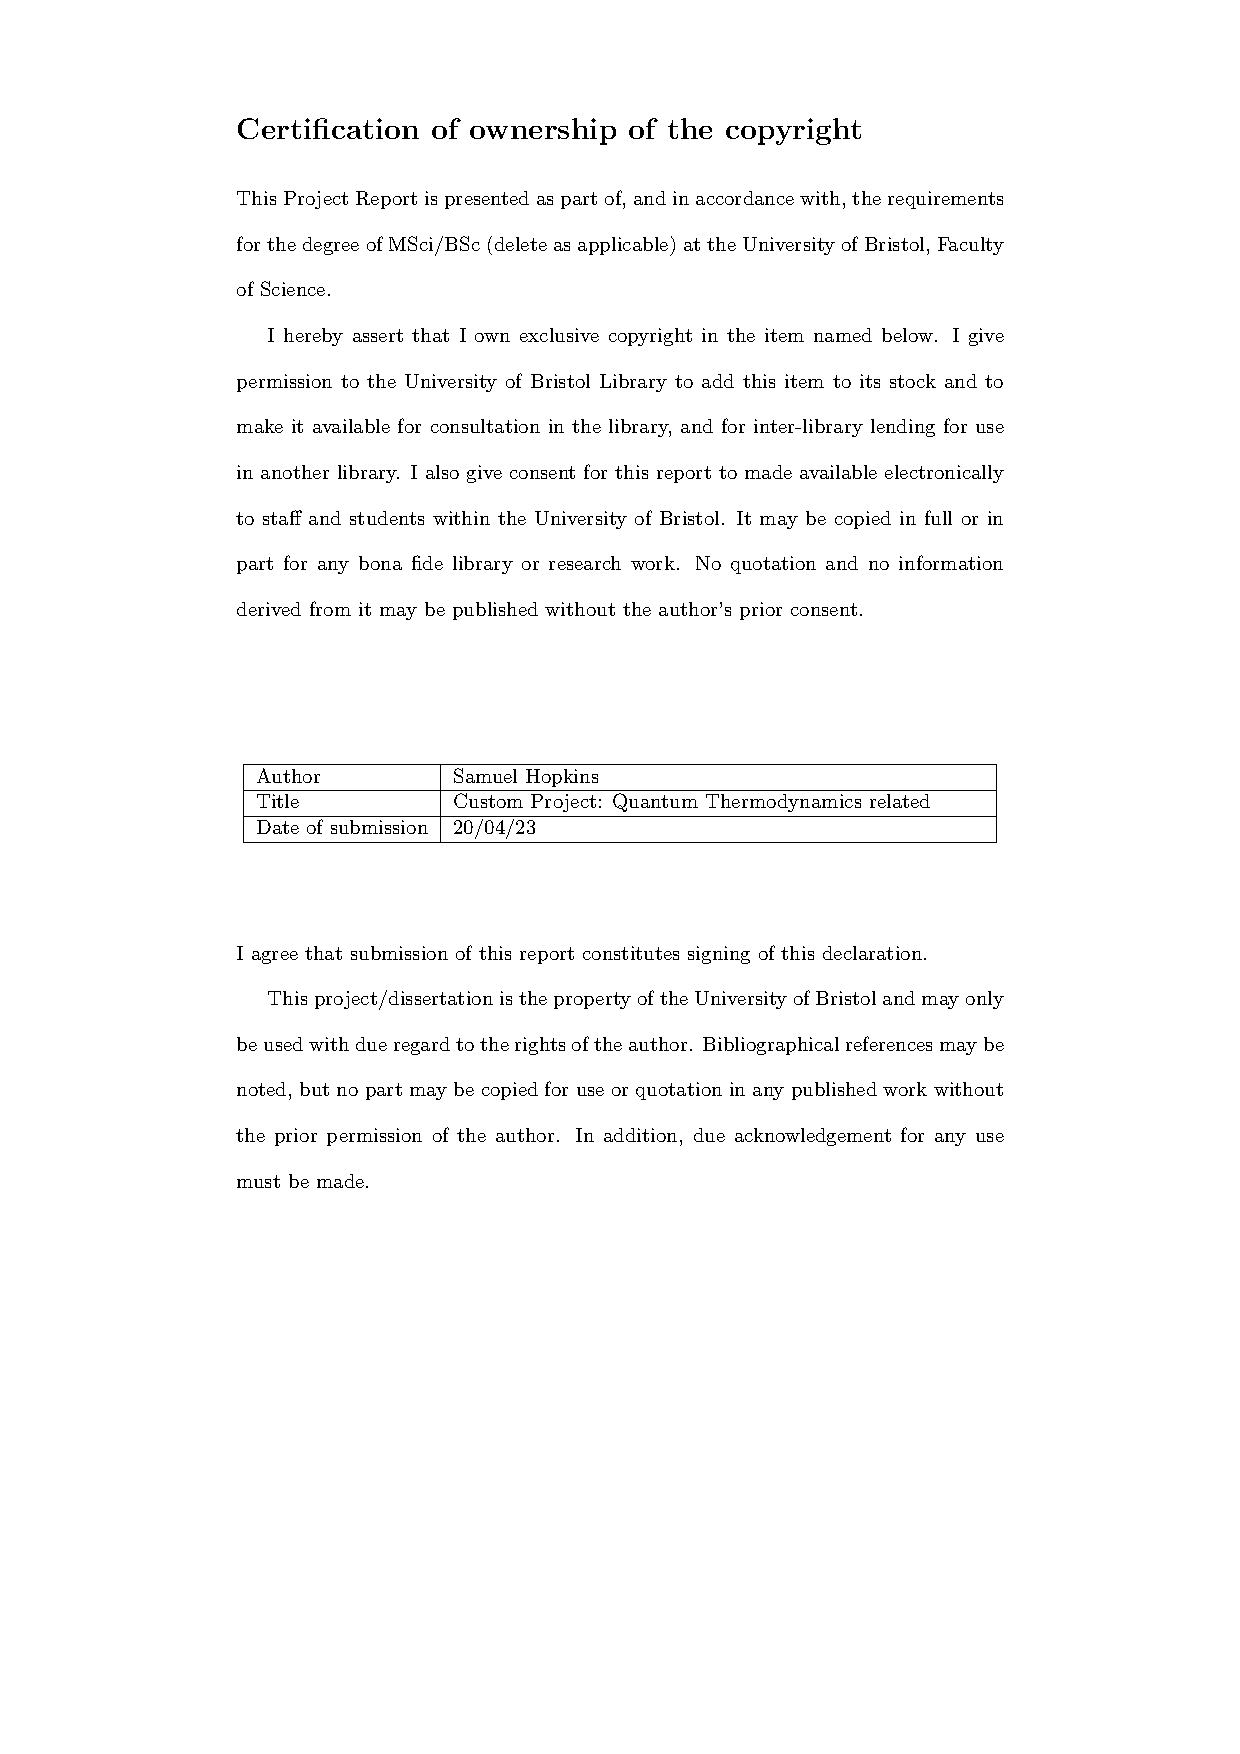
\includegraphics[width = \textwidth]{certi.pdf}


\end{document}